\section{Results and Discussion}

\subsection*{Public Dataset: COLO}

The COLO dataset contains 1,254 images and 11,818 cow instances captured from an indoor farm environment. The dataset is organized in YOLO and COCO formats and published on the online platforms GitHub \href{https://github.com/Niche-Squad/COLO/}{(https://github.com/Niche-Squad/COLO/)} and Huggingface \href{https://huggingface.co/datasets/Niche-Squad/COLO}{(https://huggingface.co/datasets/Niche-Squad/COLO)}. The dataset consists of six configurations (\textbf{Table~\ref{tab:colo_config}}):
\textit{0\_all}, \textit{1\_top}, \textit{2\_side}, \textit{a1\_t2s}, \textit{a2\_s2t}, \textit{b\_light}, \textit{ext\_VT}, and \textit{ext\_IMU}. The \textit{0\_all} configuration serves as the baseline for this study, featuring non-overlapping training and testing images collected from both the Top-View Camera and Side-View Camera. The \textit{1\_top}, \textit{2\_side}, and \textit{ext\_VT} configurations contain images from their respective cameras. The \textit{a1\_t2s}, \textit{a2\_s2t}, and \textit{b\_light} configurations include training/testing splits for the Top2Side, Side2Top, and Day2Night scenarios, respectively. The \textit{ext\_VT} and \textit{ext\_IMU} configuration is used to evaluate the model's performance on unseen data. Both training and testing images in these configurations are collected from the same camera, but the images are different. The \textit{ext\_VT} configuration uses images from the Virginia Tech dataset, while the \textit{ext\_IMU} configuration uses images from the Inner Mongolia University dataset. 

\begin{table}[h]
    \caption{Overview of the COLO dataset configurations.}
    \centering
    \begin{tabular}{llll}
        \toprule
        \textbf{Experiment} & \textbf{Configuration (folder name)} & \textbf{Training Source} & \textbf{Testing Source} \\
        \midrule
        Study 1 and Study 2& \textit{Baseline (0\_all)} & Top-View + Side-View & Top-View + Side-View \\ [0.5ex]
         & \textit{Top2Side (a1\_t2s)} & Top-View & Side-View \\[0.5ex]
         & \textit{Side2Top (a2\_s2t)} & Side-View & Top-View \\[0.5ex]
         & \textit{Day2Night (b\_light)} & Day & Night \\[0.5ex]
        \midrule
        Study 3 & \textit{ext\_VT (ext\_VT)} & Virginia Tech & Different images, same source \\[0.5ex]
                & \textit{ext\_IMU (ext\_IMU)} & Inner Mongolia University & Different images, same source \\[0.5ex]
        \midrule
        Unused & \textit{1\_top} & Top-View & Top-View \\[0.5ex]
        & \textit{2\_side} & Side-View & Side-View \\[0.5ex]
        \bottomrule
    \end{tabular}
    \label{tab:colo_config}
\end{table}


\subsection*{Study 1: The Changes in Camera View Angles Dramatically Affect Model Performance}

Regardless of model architecture, the evaluated performance across the four configurations exhibits a consistent trend: changing the camera view from top-view to side-view results in a substantial performance drop. Using the Baseline configuration as a reference and evaluating with the $\text{mAP@{0.5:0.95}}$ metric on 500 training samples, the performance decreased by 51.6\%, 50.5\%, and 44.1\% for YOLOv11, YOLOv12, and RT-DETR, respectively. The second most significant drop was observed when switching the camera view from side-view to top-view, with performance declines of 31.4\%, 30.5\%, and 16.5\% for YOLOv11, YOLOv12, and RT-DETR, respectively. Finally, altering lighting conditions from day to night also led to a noticeable drop—approximately 10\%, though this effect was less severe compared to changes in camera view angle (\textbf{Figure~\ref{fig:study1}}).

Another noteworthy observation is that the trend of improved performance with increasing training sample size is not consistent across all model architectures. For instance, in the Day2Night configuration, both YOLOv11 and YOLOv12 showed smaller performance gains when increasing the training set from 128 to 500 samples compared to the gain from 32 to 128 samples. This suggests diminishing returns—or a saturation effect—on performance with larger training sizes. In contrast, the RT-DETR model demonstrated greater marginal improvements from 128 to 500 samples across the Day2Night, Side2Top, and Top2Side configurations than from 32 to 128 samples. Although this observation is based on limited data and context, it suggests that RT-DETR is more data-hungry than YOLOv11 and YOLOv12. This aligns with the findings of \cite{wang_towards_2022}, which report that DETR-based models generally require more data than CNN-based models like YOLO.

\begin{figure}[h]
    \centering
    
\includegraphics[width=1\textwidth]{figure_4.jpg}
    \caption{
        The generalization performance of the three model architectures, including YOLOv11, YOLOv12, and RT-DETR, is evaluated across various configurations. For each architecture, performance is averaged over its two size variants. Evaluation is based on the metric $\text{mAP@{0.5:0.95}}$ using 32, 128, and 500 training samples. Different configurations are distinguished by unique color and marker combinations. The shaded area around each line indicates two standard deviations.}
    \label{fig:study1}
\end{figure}

Despite the various challenges in adapting models from day to night conditions, the `Day2Night' configuration consistently maintains higher $\text{mAP@{0.5:0.95}}$, closely mirroring the `Baseline' configuration across all training sample sizes and model architectures. This suggests that changes in lighting have less impact on the model's ability to detect objects compared to changes in viewpoint. This robustness to lighting could be attributed to the inclusion of diverse lighting conditions in the training phase. Specifically, model performance benefited from pixel-wise augmentation techniques such as adjustments to hue, saturation, and value (HSV). These augmentations introduced a variety of color variations to the images, enhancing the model's ability to generalize across different visual conditions. Moreover, these YOLO models benefit from pre-training on the COCO dataset, which is characterized by a wide array of images with varied lighting, aiding their adaptability to shifts in light.

On the other hand, the models perform suboptimally in scenarios involving changes in viewpoint. Each new viewpoint introduces fundamentally different object features that are not replicated through standard data augmentation methods such as lighting or affine transformations. For example, when the camera is placed at a lower angle, cows are more frequently occluded by stalls and fences. These additional objects introduce variations that cannot be mitigated by augmentations in HSV space or image translation. Consequently, `Top2Side' performs the worst, as it is particularly challenging to identify cows from the side. In summary, camera view angle is crucial for model generalization, with side views being the most challenging.

% \renewcommand{\arraystretch}{0.85}
\begin{table}[ht]
    \caption{Summary of YOLOv11 results for all configurations}
    \centering
    {\footnotesize
    \begin{tabular}{llllllll}
        \toprule
        \textbf{Sample Size} & \textbf{Configuration} & \textbf{Model Size} & \textbf{mAP@0.5:0.95} & \textbf{mAP@0.5} & \textbf{Precision} & \textbf{Recall} \\
        \midrule
        32  & Baseline  & Large (56.9M) & 0.408 $\pm$ 0.022 & 0.716 $\pm$ 0.025 & 0.807 $\pm$ 0.031 & 0.625 $\pm$ 0.032 \\
            &           & Small (2.6M) & \textbf{0.444 $\pm$ 0.021} & \textbf{0.760 $\pm$ 0.017} & \textbf{0.822 $\pm$ 0.024} & \textbf{0.662 $\pm$ 0.023} \\
        \cmidrule{2-7}
            & Day2Night & Large (56.9M) & 0.355 $\pm$ 0.027 & 0.624 $\pm$ 0.037 & 0.796 $\pm$ 0.038 & 0.539 $\pm$ 0.046 \\
            &           & Small (2.6M) & \textbf{0.390 $\pm$ 0.025} & \textbf{0.673 $\pm$ 0.023} & \textbf{0.805 $\pm$ 0.032} & \textbf{0.582 $\pm$ 0.029} \\
        \cmidrule{2-7}
            & Side2Top  & Large (56.9M) & 0.124 $\pm$ 0.024 & 0.292 $\pm$ 0.063 & 0.473 $\pm$ 0.062 & \textbf{0.287 $\pm$ 0.094} \\
            &           & Small (2.6M) & \textbf{0.138 $\pm$ 0.034} & \textbf{0.301 $\pm$ 0.068} & \textbf{0.484 $\pm$ 0.082} & 0.283 $\pm$ 0.069 \\
        \cmidrule{2-7}
            & Top2Side  & Large (56.9M) & 0.051 $\pm$ 0.017 & 0.121 $\pm$ 0.034 & \textbf{0.258 $\pm$ 0.084} & 0.126 $\pm$ 0.038 \\
            &           & Small (2.6M) & \textbf{0.064 $\pm$ 0.018} & \textbf{0.147 $\pm$ 0.034} & 0.248 $\pm$ 0.100 & \textbf{0.131 $\pm$ 0.036} \\
        \midrule
        128 & Baseline  & Large (56.9M) & \textbf{0.575 $\pm$ 0.014} & 0.868 $\pm$ 0.010 & \textbf{0.899 $\pm$ 0.018} & 0.771 $\pm$ 0.019 \\
            &           & Small (2.6M) & 0.567 $\pm$ 0.014 & \textbf{0.875 $\pm$ 0.011} & 0.896 $\pm$ 0.015 & \textbf{0.788 $\pm$ 0.014} \\
        \cmidrule{2-7}
            & Day2Night & Large (56.9M) & 0.478 $\pm$ 0.015 & 0.738 $\pm$ 0.018 & 0.869 $\pm$ 0.021 & 0.638 $\pm$ 0.024 \\
            &           & Small (2.6M) & \textbf{0.488 $\pm$ 0.017} & \textbf{0.772 $\pm$ 0.019} & \textbf{0.873 $\pm$ 0.020} & \textbf{0.687 $\pm$ 0.030} \\
        \cmidrule{2-7}
            & Side2Top  & Large (56.9M) & 0.210 $\pm$ 0.039 & 0.426 $\pm$ 0.064 & 0.607 $\pm$ 0.087 & 0.387 $\pm$ 0.055 \\
            &           & Small (2.6M) & \textbf{0.245 $\pm$ 0.038} & \textbf{0.472 $\pm$ 0.063} & \textbf{0.651 $\pm$ 0.050} & \textbf{0.426 $\pm$ 0.056} \\
        \cmidrule{2-7}
            & Top2Side  & Large (56.9M) & 0.093 $\pm$ 0.022 & 0.186 $\pm$ 0.034 & 0.393 $\pm$ 0.072 & 0.164 $\pm$ 0.027 \\
            &           & Small (2.6M) & \textbf{0.103 $\pm$ 0.017} & \textbf{0.207 $\pm$ 0.028} & \textbf{0.431 $\pm$ 0.082} & \textbf{0.181 $\pm$ 0.028} \\
        \midrule
        500 & Baseline  & Large (56.9M) & \textbf{0.636 $\pm$ 0.008} & \textbf{0.932 $\pm$ 0.005} & \textbf{0.919 $\pm$ 0.011} & \textbf{0.864 $\pm$ 0.011} \\
            &           & Small (2.6M) & 0.620 $\pm$ 0.006 & 0.927 $\pm$ 0.005 & 0.910 $\pm$ 0.012 & 0.856 $\pm$ 0.012 \\
        \cmidrule{2-7}
            & Day2Night & Large (56.9M) & \textbf{0.533 $\pm$ 0.013} & 0.817 $\pm$ 0.018 & \textbf{0.880 $\pm$ 0.028} & 0.726 $\pm$ 0.026 \\
            &           & Small (2.6M) & 0.524 $\pm$ 0.015 & \textbf{0.820 $\pm$ 0.018} & 0.867 $\pm$ 0.023 & \textbf{0.733 $\pm$ 0.023} \\
        \cmidrule{2-7}
            & Side2Top  & Large (56.9M) & 0.290 $\pm$ 0.042 & 0.541 $\pm$ 0.056 & 0.663 $\pm$ 0.068 & 0.480 $\pm$ 0.049 \\
            &           & Small (2.6M) & \textbf{0.338 $\pm$ 0.030} & \textbf{0.612 $\pm$ 0.043} & \textbf{0.728 $\pm$ 0.048} & \textbf{0.547 $\pm$ 0.040} \\
        \cmidrule{2-7}
            & Top2Side  & Large (56.9M) & 0.105 $\pm$ 0.014 & 0.192 $\pm$ 0.020 & 0.413 $\pm$ 0.051 & 0.193 $\pm$ 0.018 \\
            &           & Small (2.6M) & \textbf{0.117 $\pm$ 0.015} & \textbf{0.222 $\pm$ 0.026} & \textbf{0.465 $\pm$ 0.069} & \textbf{0.210 $\pm$ 0.030} \\
        \bottomrule
    \end{tabular}
    }
    \label{tab:study1}
\end{table}

\subsection*{Study 2: A Higher Model Complexity Does Not Always Lead to Better Performance}

\begin{figure}[h]
\centering

\includegraphics[width=1\textwidth]{figure_5.jpg}
\caption{A detailed breakdown of performance by size variants within each model architecture is presented. Configurations are arranged along the rows, while columns represent the different model architectures. Statistical significance of the performance differences between the two size variants is denoted using asterisks, with the following legend: * = p < 0.05, ** = p < 0.01, and *** = p < 0.001. The solid blue line represents the large model variant, while the dashed orange line represents the small model variant. The shaded area around each line indicates two standard deviations.}
\label{fig:models}
\end{figure}

The study found that training configuration significantly influences the relationship between model complexity and performance. Challenging tasks, such as predicting images across different camera angles (e.g., Top2Side and Side2Top), revealed that smaller model variants can sometimes outperform their larger counterparts. Specifically, in four out of six comparisons across three model architectures and two camera-angle configurations, the smaller models achieved better performance. In simpler tasks, such as the Baseline configuration, performance differences were generally minimal, with the small RT-DETR variant showing a statistically significant advantage, and YOLOv11/YOLOv12 variants showing less than a 3\% difference in $\text{mAP@{0.5:0.95}}$.

These findings suggest that the relationship between model size and performance is not linear or universally consistent. Instead, it depends on task complexity and dataset characteristics. In more complex configurations, simpler models occasionally performed better, challenging the assumption that larger models are always superior.

As illustrated in Figure~\ref{fig:models}, while all studied architectures (YOLOv11, YOLOv12, and RT-DETR) generally benefit from increased parameters when trained on large-scale datasets like COCO \cite{lin2014microsoft}, this pattern does not hold in the current setting. The COCO dataset includes 80 object classes and diverse standalone images, whereas this study used a domain-specific indoor farm dataset focusing on a single class: cows. Under such narrow and homogenous conditions, larger models may not offer proportional gains, and model generalization behavior differs.

For example, the small YOLOv11n model (2.6M parameters) achieved 42.7\% $\text{mAP@{0.5:0.95}}$ with just 32 training samples—outperforming a much larger model (52.1M parameters) that achieved only 40.8\%. This advantage was especially pronounced in the Top2Side and Side2Top configurations, where YOLOv11n outperformed YOLOv11x by 1.3\% and 4.7\%, respectively, with 500 training samples.

These results underscore the value of deploying smaller models in targeted, homogeneous tasks such as cow positioning, where they offer an optimal balance between computational efficiency and prediction accuracy. They also reinforce the broader point: model selection should be tailored to the specific dataset and task, rather than relying on model complexity as a proxy for better performance. In summary, higher model complexity does not inherently guarantee improved outcomes. Instead, careful consideration of the task context and dataset is essential in selecting the most effective model architecture.

\subsection*{Study 3: The Advantages of Custom Initial Weights are Limited When the Model is Simple}

The benefits of transferring weights from a related task vary between the two evaluated datasets. On the more similar dataset, \textit{ext\_VT}, models initialized with transferred weights consistently outperformed those with pre-trained weights, with statistically significant differences except for the small YOLOv11 variant. This performance gap remained even as more data from the target environment was added. In contrast, for the more distinct \textit{ext\_IMU} dataset, where the barn setting differs considerably, the advantage of transferred weights was observed only when training data was limited (e.g., 16 images). When the sample size increased to 250, the performance difference between pre-trained and transferred weights disappeared across all model architectures.

These results suggest that transferred weights offer greater benefits when the source and target domains are closely aligned. For more divergent domains, fine-tuning from general pre-trained weights may be equally or more efficient. Additionally, simpler models gain less from custom weights, indicating that using pre-trained weights is often sufficient, avoiding the labor-intensive process of creating task-specific initializations.

\begin{figure}[h]
    \centering
    
\includegraphics[width=1\textwidth]{figure_6.jpg}
    \caption{
        Fine-tuning performance ($\text{mAP@{0.5:0.95}}$) with different initial weights. Rows represent external datasets; columns represent model architectures. Solid and dashed lines indicate transferred and pre-trained weights, respectively. Blue and orange lines denote large and small model variants. Shaded areas show two standard deviations. Asterisks indicate t-test significance of performance differences between models initialized with pre-trained weights and those using transferred weights. Statistical significance is indicated by asterisks, following this legend
        : * = p < 0.05, ** = p < 0.01, *** = p < 0.001.
    }
    \label{fig:study3}
\end{figure}


\begin{table}[ht]
    \caption{Summary of YOLOv11 results for all configurations}
    \centering
    {\footnotesize
    \begin{tabular}{lllllllll}
        \toprule
        \textbf{Sample Size} & \textbf{Config.} & \textbf{Model Szie} & \textbf{Init. Weights} & \textbf{mAP@0.5:0.95} & \textbf{mAP@0.5} & \textbf{Precision} & \textbf{Recall} \\
        \midrule
            16  & e\_IMU & Large (56.9M) & Transfered & \textbf{0.40 $\pm$ 0.03} & \textbf{0.72 $\pm$ 0.04} & \textbf{0.77 $\pm$ 0.03} & \textbf{0.62 $\pm$ 0.04} \\
                &        &               & Pre-trained & 0.33 $\pm$ 0.05 & 0.63 $\pm$ 0.08 & 0.67 $\pm$ 0.09 & 0.55 $\pm$ 0.05 \\
            \cmidrule{3-8}
                &        & Small (2.6M) & Transferred & \textbf{0.37 $\pm$ 0.02} & \textbf{0.72 $\pm$ 0.03} & \textbf{0.77 $\pm$ 0.04} & \textbf{0.62 $\pm$ 0.03} \\
                &        &               & Pre-trained & 0.34 $\pm$ 0.03 & 0.68 $\pm$ 0.04 & 0.73 $\pm$ 0.05 & 0.59 $\pm$ 0.04 \\
            \cmidrule{2-8}
                & e\_VT  & Large (56.9M) & Transferred & \textbf{0.50 $\pm$ 0.03} & \textbf{0.81 $\pm$ 0.03} & \textbf{0.83 $\pm$ 0.03} & \textbf{0.71 $\pm$ 0.04} \\
                &        &               & Pre-trained & 0.38 $\pm$ 0.03 & 0.68 $\pm$ 0.03 & 0.76 $\pm$ 0.05 & 0.58 $\pm$ 0.06 \\
            \cmidrule{3-8}
                &        & Small (2.6M) & Transferred & \textbf{0.48 $\pm$ 0.02} & \textbf{0.82 $\pm$ 0.02} & \textbf{0.82 $\pm$ 0.04} & \textbf{0.72 $\pm$ 0.03} \\
                &        &               & Pre-trained & 0.40 $\pm$ 0.03 & 0.73 $\pm$ 0.03 & 0.78 $\pm$ 0.04 & 0.64 $\pm$ 0.04 \\
            \midrule
            64  & e\_IMU & Large (56.9M) & Transferred & \textbf{0.49 $\pm$ 0.01} & \textbf{0.81 $\pm$ 0.01} & \textbf{0.82 $\pm$ 0.02} & \textbf{0.71 $\pm$ 0.03} \\
                &        &               & Pre-trained & 0.48 $\pm$ 0.02 & 0.79 $\pm$ 0.01 & 0.81 $\pm$ 0.03 & 0.70 $\pm$ 0.03 \\
            \cmidrule{3-8}
                &        & Small (2.6M) & Transferred & 0.44 $\pm$ 0.01 & \textbf{0.79 $\pm$ 0.01} & \textbf{0.84 $\pm$ 0.02} & \textbf{0.69 $\pm$ 0.02} \\
                &        &               & Pre-trained & \textbf{0.44 $\pm$ 0.01} & 0.78 $\pm$ 0.01 & 0.83 $\pm$ 0.03 & 0.67 $\pm$ 0.03 \\
            \cmidrule{2-8}
                & e\_VT  & Large (56.9M) & Transferred & \textbf{0.57 $\pm$ 0.01} & \textbf{0.88 $\pm$ 0.02} & \textbf{0.87 $\pm$ 0.02} & \textbf{0.80 $\pm$ 0.02} \\
                &        &               & Pre-trained & 0.53 $\pm$ 0.02 & 0.84 $\pm$ 0.01 & 0.86 $\pm$ 0.02 & 0.76 $\pm$ 0.02 \\
            \cmidrule{3-8}
                &        & Small (2.6M) & Transferred & \textbf{0.56 $\pm$ 0.01} & \textbf{0.88 $\pm$ 0.01} & 0.87 $\pm$ 0.02 & \textbf{0.80 $\pm$ 0.02} \\
                &        &               & Pre-trained & 0.53 $\pm$ 0.02 & 0.85 $\pm$ 0.01 & \textbf{0.87 $\pm$ 0.02} & 0.75 $\pm$ 0.02 \\
            \midrule
            200 & e\_IMU & Large (56.9M) & Transferred & 0.53 $\pm$ 0.01 & 0.85 $\pm$ 0.01 & \textbf{0.85 $\pm$ 0.03} & 0.77 $\pm$ 0.02 \\
                &        &               & Pre-trained & \textbf{0.54 $\pm$ 0.01} & \textbf{0.86 $\pm$ 0.01} & 0.84 $\pm$ 0.02 & \textbf{0.78 $\pm$ 0.01} \\
            \cmidrule{3-8}
                &        & Small (2.6M) & Transferred & \textbf{0.50 $\pm$ 0.01} & \textbf{0.85 $\pm$ 0.01} & \textbf{0.88 $\pm$ 0.02} & \textbf{0.76 $\pm$ 0.02} \\
                &        &               & Pre-trained & 0.49 $\pm$ 0.01 & 0.84 $\pm$ 0.01 & 0.87 $\pm$ 0.02 & 0.74 $\pm$ 0.01 \\
            \cmidrule{2-8}
                & e\_VT  & Large (56.9M) & Transferred & \textbf{0.63 $\pm$ 0.01} & \textbf{0.91 $\pm$ 0.01} & \textbf{0.89 $\pm$ 0.02} & \textbf{0.85 $\pm$ 0.01} \\
                &        &               & Pre-trained & 0.62 $\pm$ 0.01 & 0.90 $\pm$ 0.01 & 0.89 $\pm$ 0.02 & 0.84 $\pm$ 0.02 \\
            \cmidrule{3-8}
                &        & Small (2.6M) & Transferred & 0.61 $\pm$ 0.01 & \textbf{0.91 $\pm$ 0.01} & \textbf{0.90 $\pm$ 0.02} & \textbf{0.84 $\pm$ 0.02} \\
                &        &               & Pre-trained & \textbf{0.61 $\pm$ 0.01} & 0.90 $\pm$ 0.01 & 0.89 $\pm$ 0.02 & 0.83 $\pm$ 0.02 \\
        \bottomrule
    \end{tabular}
    }
    \label{tab:study3}
\end{table}


\subsection*{Computational Resource Requirements}

\begin{figure}[h]
    \centering
    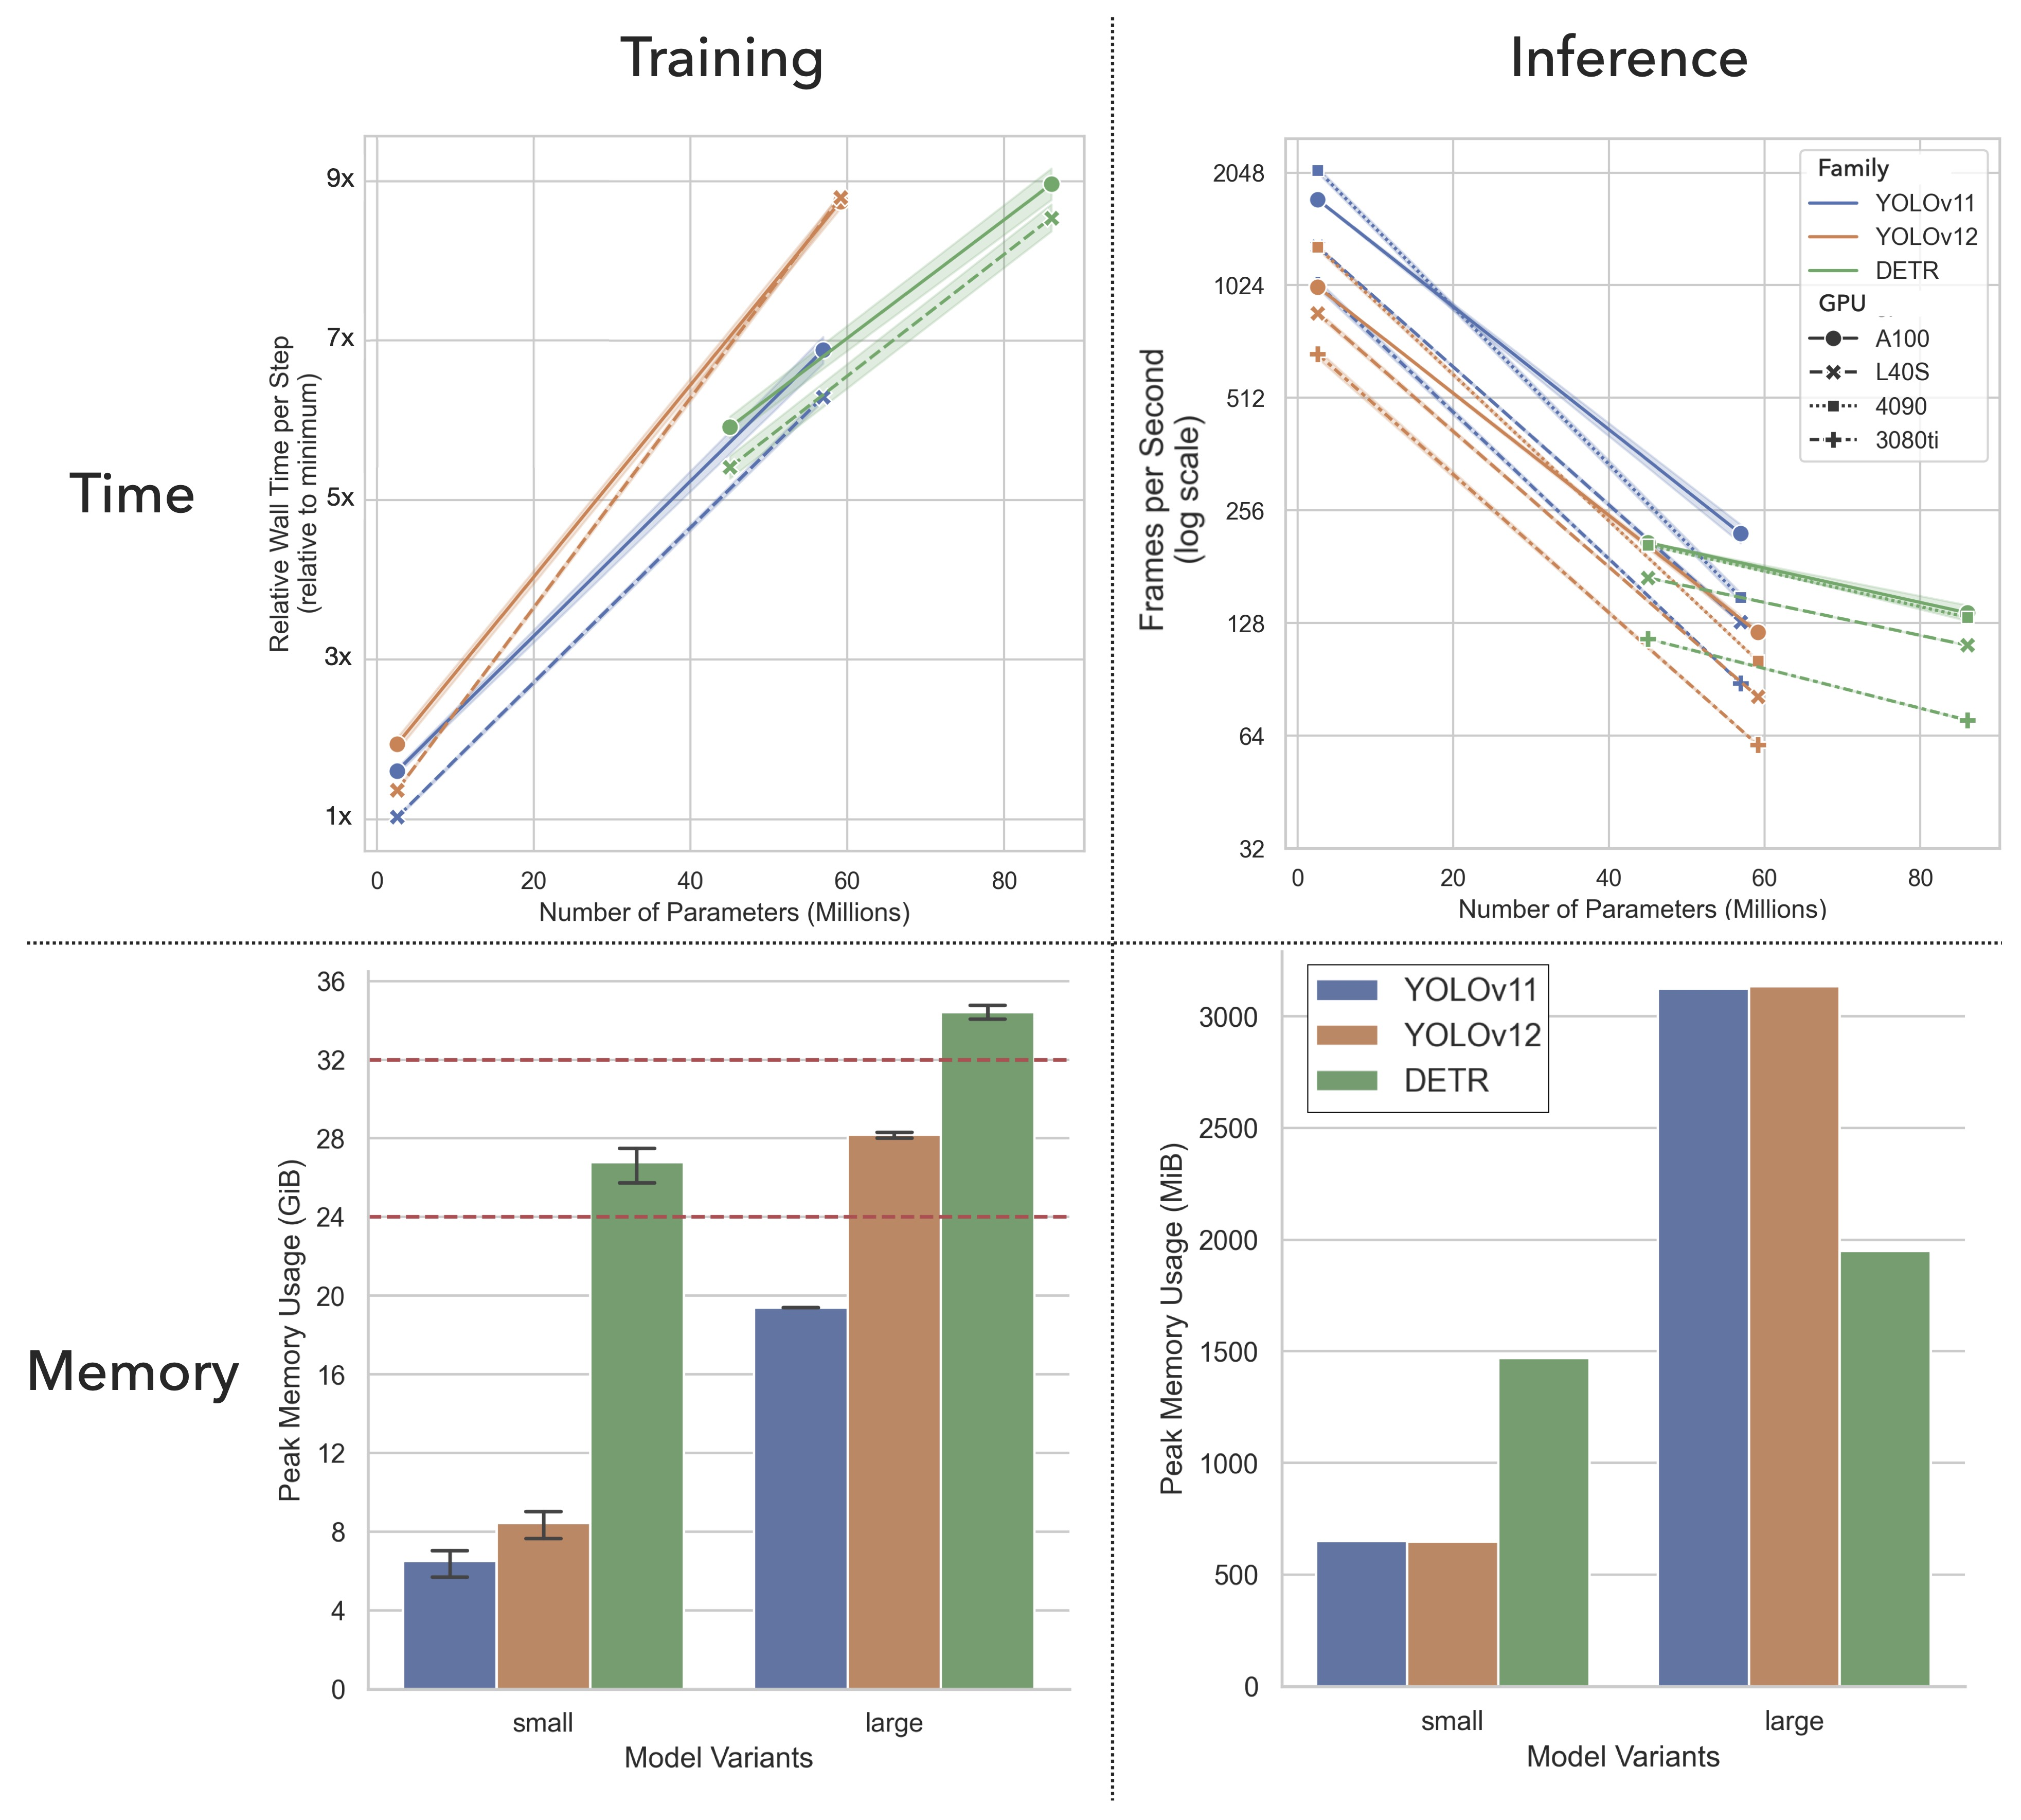
\includegraphics[width=.8\textwidth]{figure_7.jpg}
    \caption{Comparative evaluation of computational resource requirements. (Top-left) Relative training time per step with 0.6 seconds as a baseline 1x. (Top-right) Inference time in frames per second for a batch of 16 images. (Bottom-left) GPU memory peak usage during training. (Bottom-right) GPU memory peak usage during inference. The red dashed lines in the bottom left panel indicates two common GPU memory sizes of consumer-grade GPUs.}
    \label{fig:resources}
\end{figure}

\begin{table}[ht]
    \caption{Training time and memory usage for each model (mean~$\pm$~std).}
    \centering
    {\footnotesize
    \begin{tabular}{l l r r r r}
        \toprule
        \textbf{Model size} & 
        \textbf{Model} & 
        \textbf{\makecell{Params.\\(M)}} &
        \textbf{\makecell{Time per step (sec.) \\ A100 (80 GB)}} &
        \textbf{\makecell{Time per step (sec.)\\ L40S (48 GB)}} &
        \textbf{\makecell{Peak memory \\ (GiB)}}
        \\
        \midrule
        Small & yolo11n   & 2.6  & 0.97$\pm$0.03 & 0.62$\pm$0.01 & 5.92$\pm$1.08 \\
              & yolo12n   & 2.6  & 1.17$\pm$0.06 & 0.82$\pm$0.01 & 7.67$\pm$1.21 \\
              & rtdetr-l  & 45.0 & 3.56$\pm$0.09 & 3.26$\pm$0.10 & 24.46$\pm$2.46 \\
        \midrule
        Large & yolo11x   & 56.9 & 4.14$\pm$0.11 & 3.79$\pm$0.03 & 18.08$\pm$1.00 \\
              & yolo12x   & 59.1 & 5.26$\pm$0.06 & 5.29$\pm$0.04 & 26.89$\pm$1.07 \\
              & rtdetr-x  & 86.0 & 5.39$\pm$0.13 & 5.14$\pm$0.11 & 31.60$\pm$3.18 \\
        \bottomrule
    \end{tabular}
    }
    \label{tab:train_model_comparison}
\end{table}

\begin{table}[ht]
    \caption{Inference FPS and memory usage for each model (mean~$\pm$~std).}
    \centering
    {\footnotesize
    \begin{tabular}{l l r r r r r r}
        \toprule
        \textbf{Model size} & \textbf{Model} & 
        \textbf{\makecell{Params. \\(M)}} &
        \textbf{\makecell{FPS\\A100 (80 GB)}} & 
        \textbf{\makecell{FPS\\L40S (48 GB)}} &
        \textbf{\makecell{FPS\\4090 (24 GB)}} & 
        \textbf{\makecell{FPS\\3080Ti (12 GB)}} & 
        \textbf{\makecell{Required \\ memory \\ (MiB)}}
        \\
        \midrule
        Small & yolo11n   & 2.6  & 1734.90$\pm$14.71 & 1297.60$\pm$2.25 & 2079.76$\pm$86.72 & 1030.26$\pm$67.80  & 650.00 \\
              & yolo12n   & 2.6  & 1013.95$\pm$8.37  & 862.18$\pm$36.41 & 1293.46$\pm$46.96 & 670.14$\pm$45.49  & 648.75 \\
              & rtdetr-l  & 45.0 & 210.14$\pm$0.43   & 168.98$\pm$0.06  & 206.96$\pm$1.62 & 116.14$\pm$0.13   & 1469.92 \\
        \midrule
        Large & yolo11x   & 56.9 & 222.12$\pm$33.46 & 129.08$\pm$5.66 & 149.92$\pm$11.13 & 88.38$\pm$0.31  &  3125.37 \\
              & yolo12x   & 59.1 & 120.91$\pm$6.97 & 81.30$\pm$0.53   & 101.50$\pm$1.23 & 60.48$\pm$0.54  &  3133.62 \\
              & rtdetr-x  & 86.0 & 136.31$\pm$17.64 & 111.68$\pm$0.44 & 132.64$\pm$0.53 & 70.38$\pm$0.40  &  1948.73 \\
        \bottomrule
    \end{tabular}
    }
    \label{tab:infer_model_comparison}
\end{table}



Evaluating computational resource requirements is essential for determining the feasibility of deploying object detection models in real-world scenarios, particularly in environments with limited hardware capabilities. This study examines the training time, inference performance, and memory usage of all evaluated models (\textbf{Figure~\ref{fig:resources}}).
Training time for each model was measured and expressed relative to a baseline, denoted as 1×. This baseline corresponds to the fastest observed training configuration: the YOLOv11n model running on an NVIDIA L40S GPU at 0.6 seconds per training step. Across all architectures on the same GPU, training time generally scaled linearly with the number of model parameters. An exception was observed with YOLOv12, which exhibited 29.5\% and 37.6\% longer training times compared to YOLOv11 on the A100 and L40S GPUs, respectively. This discrepancy is likely attributable to YOLOv12’s hybrid architecture, which integrates elements from both YOLOv11 and RT-DETR, resulting in additional computational complexity.
All model-GPU combinations demonstrated inference speeds exceeding 60 FPS when processing a batch of 16 images. Although there is no universally accepted definition of real-time inference, a common benchmark is the frame rate of input devices, such as cameras. Human visual perception typically requires a minimum of 30 FPS for smooth real-time experiences. Thus, all models evaluated in this study meet or exceed this practical threshold for real-time deployment.
GPU memory usage is another critical factor in determining the compatibility of models with specific hardware. High-end consumer-grade GPUs, such as the NVIDIA 5090 with 32 GB of memory, are capable of training all models in the study except RT-DETR-x, which demands an average of 34.3 GiB of memory. For more commonly available GPUs, such as the NVIDIA 4090 with 24 GB of VRAM or 3080ti with 12 GB, certain larger models, including the RT-DETR variants and YOLOv12x, exceed feasible memory limits. These elevated memory requirements can present financial and logistical challenges for both researchers and practitioners. However, these barriers can be mitigated by selecting appropriately sized models with efficient initialization strategies. For instance, smaller models fine-tuned on related datasets can offer strong baseline performance while remaining within hardware constraints, as suggested by the findings of the Study 3.

This evaluation underscores the trade-offs between model complexity and computational efficiency. Larger models, such as advanced YOLO and DETR-based variants, offer improved accuracy at the cost of increased training time and memory consumption. By understanding these trade-offs, practitioners can make informed decisions about model selection based on their resource availability and application-specific requirements. Ultimately, balancing performance with computational feasibility is key to the successful deployment of object detection models in real-world settings.

\subsection*{Metric Intepretation}

\begin{figure}[h]
    \centering
    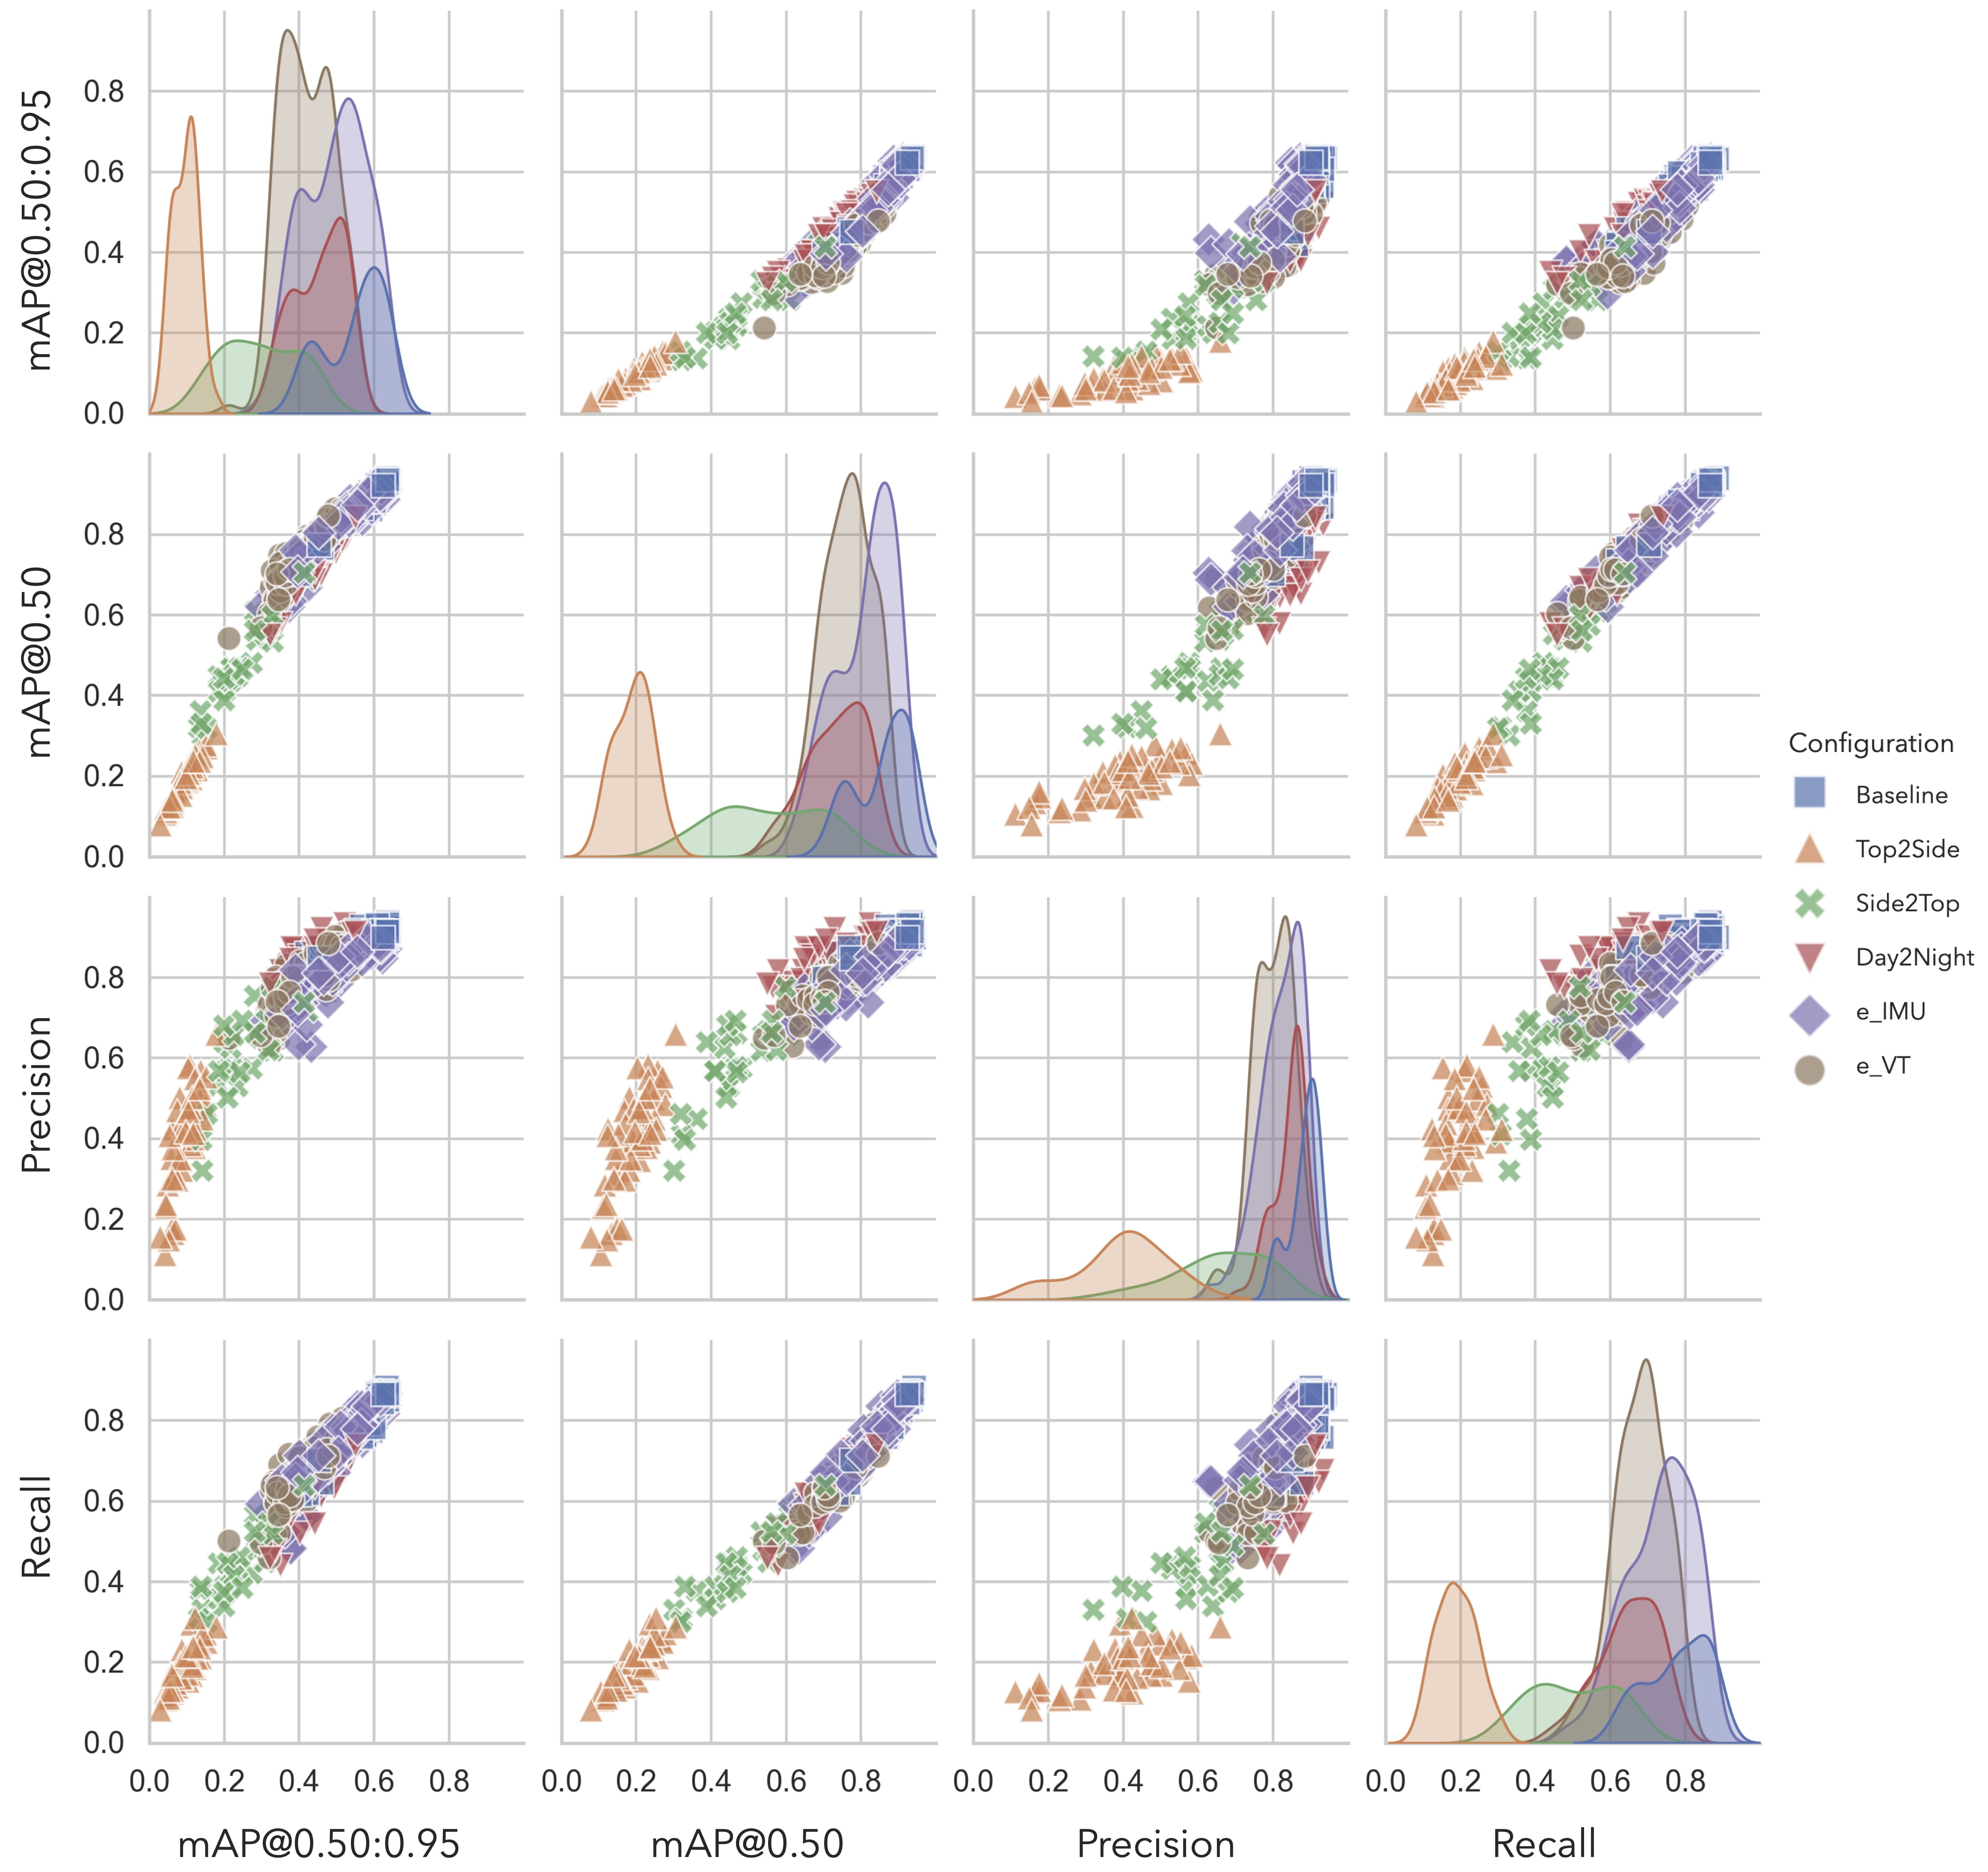
\includegraphics[width=.8\textwidth]{figure_8.jpg}
    \caption{ .}
    \label{fig:metric_interpretation}
\end{figure}


\subsection*{Study Limitations}

While this study provides multi-aspects insights into single-object detection generalization using cows as a case study, several limitations warrant consideration when interpreting the results. Firstly, the focus on a single object class, cows, inherently restricts the direct generalizability of the findings to other object categories or more complex, multi-class detection scenarios. Cows possess specific visual characteristics and appear in relatively predictable environments compared to the diversity encountered in broader object detection tasks. Consequently, the conclusion that camera angle changes pose a greater challenge than lighting variations might be specific to this context and may not hold true for objects with different textures, shapes, or typical backgrounds. Furthermore, while lighting and camera angles were investigated, other potentially significant environmental variables, such as partial occlusion (e.g., by fences, vegetation, or other animals), varying weather conditions, diverse background clutter, and significant intra-class variation (e.g., different breeds, ages, or postures of cows), were not the primary focus of the cross-validation strategies. The specific datasets used for training and validation, including their size and the diversity of conditions captured, could also influence the observed model performance and generalization capabilities.

Secondly, the investigation into model size and transfer learning, while informative, has its own constraints. The study compared a selection of model sizes and architectures; however, the findings might be dependent on the specific models chosen, and other architectures could potentially yield different results regarding robustness to the tested variations. The exploration of transfer learning demonstrated potential benefits for a similar task, but the effectiveness of transfer learning is highly contingent on the relationship between the source domain (i.e., where weights were initially trained) and the target domain (i.e., external barns), as well as the precise nature and degree of similarity of the "similar task" investigated. The performance gains observed might not be representative of transfer learning efficacy across tasks with varying degrees of relatedness or when using weights pre-trained on vastly different datasets. Additionally, the cross-validation strategies employed, while designed to isolate specific factors, represent only a subset of possible data splits and environmental challenges, and alternative validation approaches could reveal different facets of model generalization. Future work could expand the scope to include more object classes, a wider array of environmental variations and occlusions, diverse model architectures, and a more extensive analysis of transfer learning across different source and target task combinations to build upon the findings presented here.